%% Abschnitt1.tex
%% $Id: Abschnitt1.tex 28 2007-01-18 16:31:32Z bless $
%%

%% ==============================
%\subsection{Signal}
%% ==============================
%Ein Signal bildet eine Vibration ab. 
%Dabei besitzt ein Signal Attribute, die die obengenannte Reaktion darstellen sollten. 
%Als man sich die Einstellungsm{\"o}glichkeiten einer Vibration des Wearable genauer angeguckt hat, hat man festgestellt, dass man die L{\"a}nge und die St{\"a}rke einer Vibration einstellen kann. Das hat zur Folge, dass diese zwei Faktoren als die Attribute eines Signales benutzt wurden um eine Vibration zu repr{\"a}sentieren.

%Man stellt sich jetzt die Frage,
%Wie lang sollen die Vibrationen denn jetzt sein ? 

%Um diese Frage zu beantworten, guckt man sich anhand an dem Paper \cite{pescara2016ruttelflug} die benutzten Vibrationsl{\"a}ngen an. 
%Da wurden die Grenzen zwischen 100 und 1000ms f{\"u}r eine Vibration benutzt. Diese Werte hat man so {\"u}bernommen. Das bedeutet, ein Signal hat eine minimale L{\"a}nge von 100ms und eine maximale L{\"a}nge von 1000 ms. 

%Anhand der Hypothese der Bachelorarbeit wolle man wissen, wie gut sich personalisierte Vibrationen im Vergleich zu generischen Vibrationen verbessern. Diese Frage l{\"a}sst sich wie folgt beantworten. Erstens musste man sich {\"u}berlegen, wie man personalisierte Vibrationen mittels dem EA f{\"u}r einen Probanden bestimmen will.
%Au{\ss}erdem sollte man herausfinden was f{\"u}r Signale noch gut voneinander unterscheidbar sind, die die Grenzen von 100ms bis 1000ms besitzen.
%Man habe sich auf drei Typen von Signalen festgelegt, die als Kurz, Mittel und Lang definiert sind. Dadurch wolle man wissen, ob ein Signal als Kurz, Mittel oder Lang empfunden wurde.

%Die jeweiligen Typen definieren innerhalb der Grenzen von 100ms und 1000ms ein Intervall, die sich voneinander nicht {\"u}berschneiden kann. 
%Abgesehen davon ist der niedrigste Messwert von einem Langen Signal allgemein gr{\"o}{\ss}er als der h{\"o}chste Messwert von einem Mittleren Signal. Wiederum ist die kleinste Intensit{\"a}t von einem Mittleren Signal in der Regel gr{\"o}{\ss}er als die gr{\"o}{\ss}te Internsit{\"a}t von einem Kurzen Signal. Als Beispiel habe man f{\"u}r Kurz die Intervallgrenzen 100ms und 300ms, f{\"u}r Mittel habe man dann die Intervallgrenzen von 400ms bis 600ms und f{\"u}r Lang habe man die Intervallgrenzen von 700ms bis 1000ms. 
%Allerdings wurde es darauf geachtet, dass die Grenzen nicht aufeinander liegen, sondern einen Abstand zwischen den Grenzen existiert. 
%Bei der St{\"a}rke einer Vibration wurde man an der Darstellbarkeit des Wearable gebunden. Nachdem man herausgefunden hat, dass man nur die Bereiche von 0x7FFF bis 0xFFFF als merkbare Vibrationsst{\"a}rken besitzt, hat man sich diese Bereiche in 5 Stufen eingeteilt. Daraus folgt dass man sich f{\"u}r den sp{\"a}teren Verlauf f{\"u}nf Zust{\"a}nde definiert. 

%\begin{tabular}{lcr}
%  Signalst{\"a}rke & Namen & Zustandsnamen \\
%  $\mathtt{0x7FFF}$ & Very Weak & $q_{VWeak}$ \\
%  $\mathtt{0x9FFF}$ & Weak & $q_{Weak}$ \\
%  $\mathtt{0xBFFF}$ & OK & $q_{OK}$ \\
%  $\mathtt{0xDFFF}$ & Strong & $q_{Strong}$ \\
%  $\mathtt{0xFFFF}$ & Very Strong & $q_{VStrong}$ \\
%\end{tabular}

%% ==============================
%\subsection{Eingabe f{\"u}r den Algorithmus}
%% ==============================
\paragraph{Grenzen Initialisieren}
Als Eingabe f{\"u}r den Algorithmus ben{\"o}tigt man eine Start Population / Anfangspopulation von Individuen. Die Individuen sind in diesem Fall Signale. 
Nicht jede Person empfindet ein vorgegebenes Kurzes Signal gleich wie eine andere Person, somit musste man zuvor den Benutzer befragen, was er als Kurz, Mittel und Lang empfindet. Zuerst habe man alle Signale abgespielt, damit der Proband wusste, was Ihn erwartet. 
Nachdem alle Signale abgespielt wurden, wurde jedes Signal einzeln abgespielt und der Proband hatte die Aufgabe das abgespielte Signal der Kategorie Kurz, Mittel oder Lang zuzuordnen. 
Jedem Probanden wurde insgesamt 10 Signale mit der gleichen Vibrationsst{\"a}rke abgespielt, die Signalel{\"a}nge ist dabei gleich verteilt.
Dabei wurden alle 10 Signale in einer zuf{\"a}lligen Reihenfolge abgespielt.

Nach der Eingabe des Probanden erh{\"a}lt man beispielsweise folgende Bewertung \autoref{idealeingabe} erhalten. Diese Eingabe ist ideal, da alle Signaltypen direkt hintereinander vorliegen, so w{\"u}rde man hier einfach die Grenzen aus der Tabelle entnehmen k{\"o}nnen. Diese belaufen sich f{\"u}r Kurz zwischen 100 und 300 ms, f{\"u}r Mittel zwischen 400ms und 600ms und f{\"u}r Lang zwischen 700 und 1000ms.

\begin{table}[]
\centering
\caption{Bewertung eines Probanden die Ideal ist. Dabei ist die \textit{L{\"a}nge} die Signall{\"a}nge in ms und \textit{Erkannt} ist das erkannte Signal durch dem Benutzer }
\label{idealeingabe}
\resizebox{\linewidth}{!}{%
\begin{tabular}{l|l|l|l|l|l|l|l|l|l|l}
%\hline
 L{\"a}nge & 100 & 200 & 300 & 400 & 500 & 600 & 700 & 800 & 900 & 1000 \\ \hline
 Erkannt & Kurz & Kurz & Kurz & Mittel & Mittel & Mittel & Lang & Lang & Lang & Lang \\ %\hline
\end{tabular}}
\end{table}

Falls die Eingabe jedoch nicht so Ideal sein sollte, wie im Beispiel \autoref{nichtidealeeingabe}, mussten ein paar Vorkehrungen getroffen werden. Um einige Sonderf{\"a}lle auszuschlie{\ss}en, hat man {\"u}berpr{\"u}ft, ob das Signal mit der L{\"a}nge von 100ms ein Kurzes Signal ist und das Signal mit der L{\"a}nge von 1000ms ein Langes Signal ist, sowie man annimmt, dass mindestens jeder Signaltyp mindesten zwei mal ausgew{\"a}hlt wurde. Sollte dies nicht der Fall sein, so w{\"u}rde man den Benutzer dazu bitten, die zehn Signale erneut zu bewerten. 

\begin{table}[]
\centering
\caption{Bewertung eines Probanden die nicht Ideal ist. Dabei ist die \textit{L{\"a}nge} die Signall{\"a}nge in ms und \textit{Erkannt} ist das erkannte Signal durch dem Benutzer}
\label{nichtidealeeingabe}
\begin{tabular}{l|l|l|l|l|l|l|l|l|l|l}
%\hline
 L{\"a}nge & 100 & 200 & 300 & 400 & 500 & 600 & 700 & 800 & 900 & 1000 \\ \hline
 Erkannt & Kurz & Kurz & Mittel & Mittel & Lang & Mittel & Lang & Lang & Lang & Lang \\ %\hline
\end{tabular}
\end{table}

Man beginnt damit die neuen Intervallgrenzen zu bestimmen. Diese wurden anhand des Beispiels \autoref{bestimmunggrenzen} exemplarisch bestimmt, dabei ist jede Spalte eine Iteration. Dabei bestimmt man zuerst den kleinsten Wert und setzt den f{\"u}r alle Grenzen gleich. Falls ein gr{\"o}{\ss}erer Wert des f{\"u}r den gleichen Signaltypen existiert, erhalten alle nachfolgenden Grenzen den gleichen Wert zugewiesen. Wenn f{\"u}r den n{\"a}chsten Signaltyp ein gr{\"o}{\ss}erer Wert vorliegt werden nur noch die nachfolgenden Signaltypen nach diesem Wert angepasst. Nachdem die 10 Iterationen ausgef{\"u}hrt sind, untersucht man, ob die Grenzen nicht identisch sind und ob die Grenzen jeweils aufsteigend sind. \\

$Kurz_{Min} \textless Kurz_{Max} \textless Mittel_{Min} \textless Mittel_{Max} \textless Lang_{Min} \textless Lang_{Max}$ \\

Falls dies nicht der Fall sein sollte, dann wird der Benutzer erneut aufgefordert die 10 Signale zu bewerten.

\begin{table}[]
\centering
\caption{Bestimmung der Grenzen}
\label{bestimmunggrenzen}
\begin{tabular}{l|l|l|l|l|l|l|l|l|l}
%\hline
Iterationen            & 1. & 2. & 3. & 4. & 5. & 6. & 7. & 8. & 10. \\ \hline
$Kurz_{Min}$   & 100          & 100          & 100          & 100          & 100          & 100          & 100          & 100          & 100           \\ \hline
$Kurz_{Max}$   & 100          & 200          & 200          & 200          & 200          & 200          & 200          & 200          & 200           \\ \hline
$Mittel_{Min}$ & 100          & 200          & 300          & 300          & 300          & 300          & 300          & 300          & 300           \\ \hline
$Mittel_{Max}$ & 100          & 200          & 300          & 400          & 400          & 600          & 600          & 600          & 600           \\ \hline
$Lang_{Min}$   & 100          & 200          & 300          & 400          & 500          & 600          & 700          & 700          & 700           \\ \hline
$Lang_{Max}$   & 100          & 200          & 300          & 400          & 500          & 600          & 700          & 800          & 1000          \\ %\hline
\end{tabular}
\end{table}

Bei einer kleinen Abweichung von zwei nebeneinanderliegen von zwei Werten ist dies noch akzeptabel, bei gr{\"o}{\ss}eren Abweichungen, hat man Benutzer noch einmal darum gebeten erneut zu bewerten. Im Verlauf der Studie musste man nur 15\% aller Probanden ein weiteres mal darum bitten, die Signale neu zu bewerten. 

\paragraph{Population}

Sind die Grenzen f{\"u}r eine Probanden bestimmt, kann darauffolgend die Startpopulation erzeugt werden.
%Nachdem man jetzt die Grenzen f{\"u}r einen Probanden bestimmt hat, kann man die Startpopulation des Algorithmus erzeugen. 
Bei der \textbf{Startpopulation} hat man f{\"u}r jeden Signaltypen zehn Signale. 
Zwei Signale der zehn Signale repr{\"a}sentieren das Minimum und das Maximum des jeweiligen Signaltypen.
Die restlichen acht Signale erhalten eine zuf{\"a}llige L{\"a}nge innerhalb des Intervalls. Die St{\"a}rke eines Signal wird zuf{\"a}llig f{\"u}r jedes Signal zuf{\"a}llig zugewiesen. 
Man besitzt somit f{\"u}r die Startpopulation drei{\ss}ig Signale, die jeweils in zehn Kurze, Mittlere und Lange Signale unterteilt sind. 

An dieser Stelle muss man besonders betonen, dass man nur beim ersten mal eine \textbf{Startpopulation} erzeugt. 
F{\"u}r die Erzeugung der Populationen f{\"u}r die n{\"a}chsten Generationen werden die Grenzen der Signaltypen nicht explizit hinzugef{\"u}gt. 

%Anhand dem Verfahren hat man nur eine grobe Unterteilung, deswegen {\"u}berpr{\"u}ft man, ob diese grobe Absch{\"a}tzung passt.
%Zun{\"a}chst bestimmt man f{\"u}r jeden Signaltypen das arithmetische Median, was in diesem Fall 150 f{\"u}r Kurz, 433 f{\"u}r Mittel und 780 f{\"u}r Lang ist.
%Da sich die Grenzen vom Minimum von Kurz und das Maximum von Lang nicht {\"a}ndern, sind $Kurz_{Min}$ = 100ms und $Lang_{Max}$ = 1000ms bei jedem Probanden fest definiert und beginnt damit f{\"u}r Kurz und Lang die Grenzen zu bestimmen.
%Zuerst berechnet man anhand der groben Absch{\"a}tzung der Grenzen den Mittelwert, dabei ergibt sich $Kurz_{Mit}$ = 150 und $Lang_{Mit}$ = 850.

%Wenn das arithmetische Median kleiner als der Mittelwert ist, dann berechnet man bei Kurz ein neues Maximum und bei Lang ein neues Minimum.
%Bei Kurz ist dies nicht der Fall, da der Median und Mittelwert beide 150 sind, daher bleibt $Kurz_{Max}$ = 200ms.
%Bei Lang tritt dieser Fall ein und daher berechnet anhand der Formel $Lang_{Min} = (2 * Lang_{Med}) - Lang_{Max}$ daraus ergibt sich f{\"u}r $Lang_{Min}$ = 560. 

%W{\"u}rden sich die erkannten Signaltypen {\"u}berschneiden, so f{\"a}ngt man an das arithmetische Mittel von Kurz, Mittel und Lang zu bilden; desweiteren werden neue Grenzen bestimmt, indem man von der kleinsten Signall{\"a}nge anf{\"a}ngt und diese dann dem zuwei{\ss}t, was ausgew{\"a}hlt worden ist. Man hat drei mal das Minimum und das Maximum von Kurz, Mittel und Lang, die neu bestimmt werden, dabei wird anhand der folgenden Tabelle gezeigt, wie die neuen Intervalle bestimmt werden.


%Da man wei{\ss}, dass das Minimum von Kurz 100ms und das Maximum von Lang 1000ms ist, berechnet man die Intervalle von Kurz und Lang zuerst. Dabei berechnet man den Mittelwert um herauszufinden, ob das arithmetische Mittel identisch mit dem Mittel wert ist. Wenn dies der Fall ist, so sind die Grenzen f{\"u}r den Fall richtig und es muss f{\"u}r den Signaltypen nichts weiter berechnet werden. 

%Da man wei{\ss}, dass das Minimum von Kurz 100 ms und das Maximum von Lang 1000ms ist, berechnet man die Differenz zwischen dem  und dem Minimum von Kurz. Diese Differenz auf das Median dazu addiert und {\"u}berpr{\"u}ft, ob 


%% ==============================
\paragraph{Bewertung des Algorithmus}
%% ==============================

Jedes Individuum einer Population muss vor der Ausf{\"u}hrung des n{\"a}chsten Schritts des Algorithmus bewertet werden.
Um diese Bewertung zu erhalten h{\"a}tte man aus einigen Alternativen w{\"a}hlen k{\"o}nnen wobei ich hier ein weiteres erl{\"a}utern werde und wieso man dieses nicht gew{\"a}hlt hat. 

Zuerst k{\"o}nnte man hergehen und jedes Signal aus der Population dem Probanden abspielen und fragen was f{\"u}r ein Signaltyp er erkannt hat, wie man es bei den ersten zehn Signalen gemacht hat um die Grenzen der Signaltypen zu bestimmen. 

Der erste Ansatz w{\"a}re man w{\"u}rde die Anzahl der richtigen Zuweisungen und Abweichungen z{\"a}hlen um mit einer geeigneten Fitnessfunktion den Fitnesswert zu bestimmen. Ferner w{\"u}rde das bedeuten, dass f{\"u}r eine Population ein Individuum mehrmals abgespielt werden m{\"u}sse, um eine Bewertung des einzelnen Individuums zu erhalten. Bei einer Annahme von f{\"u}nf Bewertungen pro Individuum, um nur eine Population damit bewerten zu k{\"o}nnen, m{\"u}sste der Proband eine Anzahl von 150 Signalen bewerten, damit der Algorithmus eine Generation bestimmen kann. Dies w{\"u}rde bedeuten, dass wenn man vier Generationen bestimmen wollen w{\"u}rde, man auf eine Anzahl von 600 Vibrationen kommt, die der Benutzer bewerten sollte um einen personalisierten Wert zu erhalten. 
% Bewertungen alleine f{\"u}r die Bestimmung des personalisierten Wertes mithilfe dem EA. 

Aufgrund der Tatsache, dass Probanden nicht so lange an einer freiwilligen Studie teilnehmen wollen, habe man sich f{\"u}r einen anderen Ansatz entschieden. Man muss akzeptieren, dass man {\"u}ber mehrere Generationen hinweg die komplette Population bewerten muss. Das hei{\ss}t, dass man pro Generation 30 Signale abspielen muss. Um eine Generation zu bestimmen habe man sich Gedanken dar{\"u}ber gemacht, wie man so ein Signal bewerten soll. Dabei ist man zu dem Entschluss gekommen, dass man den Benutzer zuerst fragt, was f{\"u}r ein Signaltyp er erkannt habe. Weiterhin habe man Ihn zwei Fragen wie in einem Fragebogen (Likert-Skala) gestellt, wie gut er das Signal erkannt hat und wie man die St{\"a}rke des Signals empfand. 

Wie schon erw{\"a}hnt hat jedes Individuum einer Population eine zuf{\"a}llige St{\"a}rke zugewiesen.
% f{\"u}r die Population hat jedes Individuum eine zuf{\"a}llige St{\"a}rke zugewiesen. 
Dabei entspricht die St{\"a}rke einem Zustand aus dem Zustandsdiagramm \autoref{zdiagramm}, der in der ersten Population zuf{\"a}llig bestimmt worden ist, weshalb auch kein Startpunkt zusehen ist, da jeder Zustand der Startzustand sein kann. Anhand der Bewertung auf die Frage, wie man die St{\"a}rke empfunden hat, ver{\"a}ndert sich der aktuelle Zustand der St{\"a}rke eines aktuellen Individuums um bis zu zwei Zust{\"a}nde. Dabei ist die Wertigkeit der Antwort in der Tabelle \autoref{bewertungzdiagrammfrage} beschrieben. 
Die Bewertung +2 bedeutet, dass ein Zustandswechsel des aktuellen Zustands um zwei Zust{\"a}nde passiert. 
Um es an einem Beispiel zu erkl{\"a}ren, nehmen wir an, dass der Startzustand $q_{0}$ ist. Dem Probanden w{\"u}rde jetzt ein Signal mit der St{\"a}rke $\mathtt{0x7FFF}$ abgespielt. Wenn der Benutzer jetzt auf die Frage mit \textbf{zu schwach} beantwortet h{\"a}tte, wechselt der Zustand jetzt zu $q_{2}$. Wenn man immer noch von dem Zuf{\"a}lligen Startzustand von $q_{0}$ ausgeht und der Proband nach dem abspielen des Signals mit einer der Antworten \textbf{ok}, \textbf{stark} oder \textbf{zu stark} antworten w{\"u}rde, w{\"u}rde es keine {\"a}nderung des Zustandes geben, da es keine schw{\"a}chere St{\"a}rke existiert. Die Ausgabe des Zustandsdiagramms ist die Signalst{\"a}rke die in der Tabelle \autoref{belegungzdiagramm} steht. Es wird zu jedem Zustand eine andere Signalst{\"a}rke abgespielt. Diese {\"a}nderung erfolgt direkt nach der Beantwortung des Signals. 

\begin{figure}
	\centering
    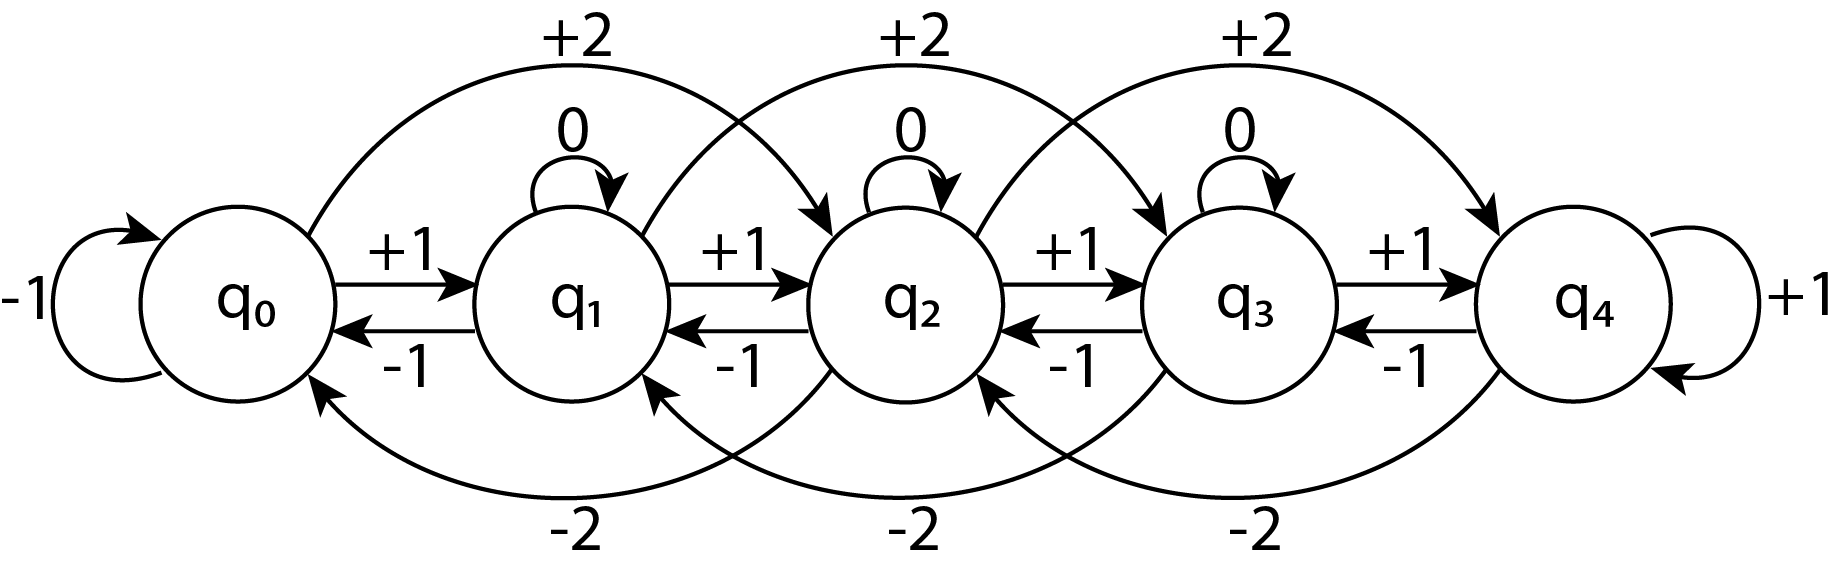
\includegraphics[width=0.9\textwidth,height=3.5cm]{pics/entwurf/zdiagramm3.png}
    \caption{Zustandsdiagramm f{\"u}r die St{\"a}rke}
    \label{fig:zdiagramm}
\end{figure}

\begin{table}[]
\centering
\caption{Signalst{\"a}rke}
\label{belegungzdiagramm}
\begin{tabular}{l|l|l}
  Signalst{\"a}rke  & Namen       & Zustandsnamen \\ \hline
  $\mathtt{0x7FFF}$ & Very Weak   & $q_{0}$       \\ \hline
  $\mathtt{0x9FFF}$ & Weak        & $q_{1}$       \\ \hline
  $\mathtt{0xBFFF}$ & OK          & $q_{2}$       \\ \hline
  $\mathtt{0xDFFF}$ & Strong      & $q_{3}$       \\ \hline
  $\mathtt{0xFFFF}$ & Very Strong & $q_{4}$       \\
\end{tabular}
\end{table}

\begin{table}[]
\centering
\caption{Bewertung der Frage, wie man die St{\"a}rke empfunden hat}
\label{bewertungzdiagrammfrage}
\begin{tabular}{l|l|l|l|l|l}
Antwort    & zu schwach              & schwach                 & ok                     & stark                   & zu stark               \\ \hline
Wertigkeit & \multicolumn{1}{c|}{+2} & \multicolumn{1}{c|}{+1} & \multicolumn{1}{c|}{0} & \multicolumn{1}{c|}{-1} & \multicolumn{1}{c}{-2}
\end{tabular}
\end{table}

Anhand der Frage, was f{\"u}r ein Signal erkannt wurde, ist f{\"u}r das Programm irrelevant gewesen. Diese Information sollte f{\"u}r die Bewertung der Studie dienen.
%Die Antwort was f{\"u}r ein Signal erkannt wurde zeigt, was f{\"u}r ein Signal der Proband erkannt hat. Dies ist f{\"u}r die Bewertung der Studie hilfreich.

Mittels der letzten Frage, wie gut ein Proband das Signal erkannt hat, hat man einen Wert hinter jeder Antwortm{\"o}glichkeit gelegt. Die Antwort auf die Frage repr{\"a}sentiert den Fitnesswert. 
%Die letzte Frage die der Benutzer zu beantworten hat, wie er das Signal erkannt hat, hat die Wertigkeit wie in Tabelle XA definiert. Diese Antwort auf die Frage, ist der entscheidende Wert, der den Fitnesswert repr{\"a}sentiert. 

\begin{table}[]
\centering
\caption{Bewertung der Frage, wie gut man das Signal erkannt hat.}
\label{signalRating}
\begin{tabular}{l|l|l|l|l|l}
Antwort   & sehr schlecht          & schlecht               & ok                    & gut                   & sehr gut              \\ \hline
Wertigkeit & \multicolumn{1}{c|}{1} & \multicolumn{1}{c|}{2} & \multicolumn{1}{c|}{3} & \multicolumn{1}{c|}{4} & \multicolumn{1}{c}{5}
\end{tabular}
\end{table}

%% ==============================
\paragraph{Erzeugung der n{\"a}chsten Generation}
%% ==============================
Im Anschluss nach der Bewertung erfolgt die Bestimmung der n{\"a}chsten Generation. Dies erfolgt mit der Selektion, Rekombination und Mutation der Gene. 

%% ==============================
\paragraph{Selektion}
%% ==============================
F{\"u}r die Selektion wird f{\"u}r jeden Signaltyp ein neuer Pool erzeugt. 
F{\"u}r jeden Signaltypen bestimmt man das Maximum $Fitness_{Max}$ von allen Fitnesswerten.
%Im Anschluss daran werden die drei Maxima f{\"u}r jeden Signaltypen von allen Fitnesswerten bestimmt. 
Anhand der Formel 
 %
\begin{equation}
  \text{H{\"a}ufigkeit} = \frac {\text{Fitnesswert eines Individuums}} {\text{$Fitness_{Max}$ des Signaltypens}}\cdot 100
\end{equation}
 %
%$(Fitnesswert eines Individuums / Maximum des zugeh{\"o}rigen Signaltypens) * 100$ 

l{\"a}sst sich die H{\"a}ufigkeit bestimmen, wie oft ein Individuum in den Pool hinzugef{\"u}gt wird. Als Beispiel hat man ein Maximum von 5 und einen Fitnesswert von 2, daraus ergibt sich 40; das hei{\ss}t, es wird 40 mal das jeweilige Individuum in den Pool hinzuf{\"u}gt. Dabei wird jedes Individuum in das Pool hinzugef{\"u}gt, welchem Signaltyp es angeh{\"o}rt. 

Nach der Erzeugung der Pools wird eine Rekombination durch zwei zuf{\"a}llig ausgew{\"a}hlte Individuen ausgef{\"u}hrt.


%% ==============================
\paragraph{Rekombination}
%% ==============================
In der Rekombination wurden die zwei zuf{\"a}llig ausgew{\"a}hlten Individuen als Eltern definiert. Die gefundenen Eltern erzeugen ein neues Individuum, dass in die Population der n{\"a}chsten Generation hinzugef{\"u}gt wird. 

Dieser Vorgang wurde wie folgt f{\"u}r das Problem angepasst. Man hat die zwei Gene, die St{\"a}rke und die L{\"a}nge eines Signals.

Zuerst beginnen wir mit der L{\"a}nge des Signals. Es wird die L{\"a}nge des ersten Elternteils und die L{\"a}nge des zweiten Elternteils genommen und ein Mittelwert von beiden Werten gebildet. Der Mittelwert ist die L{\"a}nge des neuen Individuums.
Bei der St{\"a}rke wurde direkt nach der Beantwortung des Signals die St{\"a}rke angepasst. Dieser Angepasste St{\"a}rke wert wird von beiden Elternteilen genommen und man bildet aus beiden ebenfalls den Mittelwert und rundet diesen ab.
%F{\"u}r die St{\"a}rke des neuen Individuums wird ebenfalls der Mittelwert von beiden Elternteilen gebildet und abgerundet.

Aus jedem der drei erzeugten Pools werden zehn neue Individuen f{\"u}r die n{\"a}chste Generation erzeugt, so dass man wieder auf eine Gesamtzahl von 30 Individuen f{\"u}r eine Population kommt.


%% ==============================
\paragraph{Mutation}
%% ==============================
Es besteht eine Chance von 5\% dass sich ein Individuum mutieren kann. Das bedeutet in diesem Fall, dass sich lediglich die L{\"a}nge zuf{\"a}llig ver{\"a}ndern kann. 

%% ==============================
\paragraph{Abbruchkriterium}
%% ==============================
%\begin{figure}
%	\centering
%    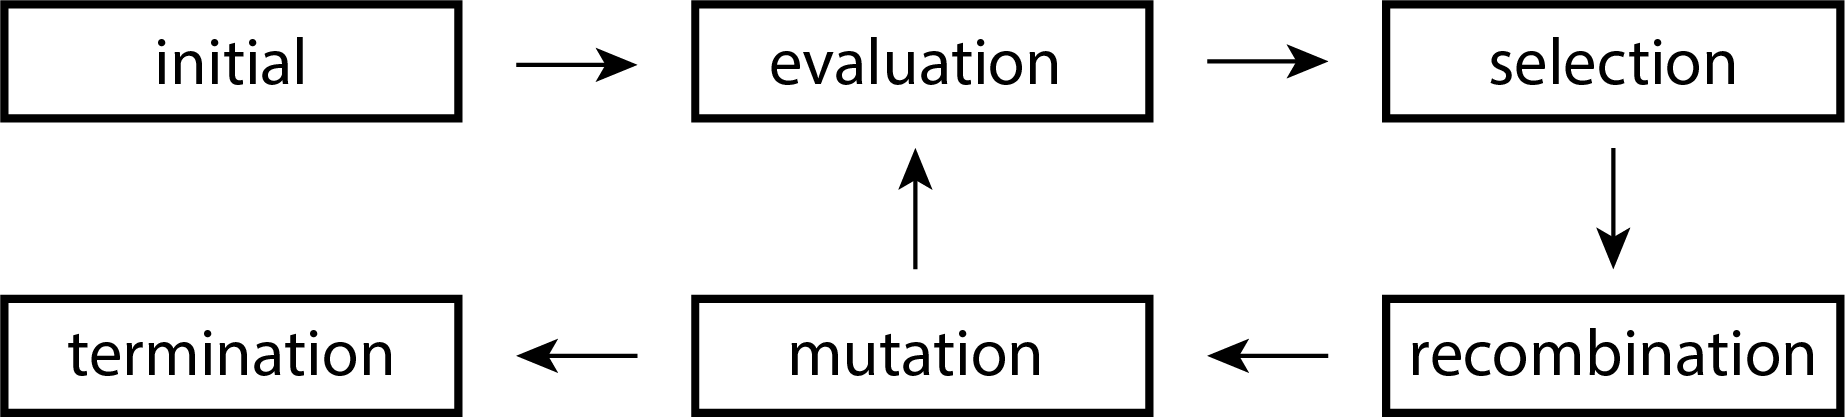
\includegraphics[width=\textwidth]{pics/algo.png}
%    \caption{Ablauf des Algorithmus}
%    \label{fig:ablaufalgo}
%\end{figure}

Man wiederholt f{\"u}r jede Generation wie den Zyklus \autoref{fig:algoSchritte}, bis man eine ausreichende L{\"o}sung erh{\"a}lt.

Das Abbruchkriterium ist in diesem Fall erreicht, wenn die vierte Generation erzeugt worden ist. Um hier die Stellung zu der Entscheidung von vier Generationen zu nehmen, ist es so, dass man versucht habe die Anzahl der Vibrationen f{\"u}r einen Probanden niedrig zu belassen. Im Vergleich zum ersten Ansatz, in der man 600 Vibrationen f{\"u}r vier Generationen hat, habe man f{\"u}r die aktuell benutze L{\"o}sung bei 30 Individuen pro Population, f{\"u}r 4 Generationen, 120 Vibrationen. 

Nach dem man die letzte Population vom Algorithmus erh{\"a}lt, bestimmt man f{\"u}r jeden Signaltypen das Minimum und Maximum von der St{\"a}rke und der L{\"a}nge von allen Signalen. Anhand derer man den Mittelwert bestimmt und schlie{\ss}lich den personalisierten Wert f{\"u}r den Probanden erh{\"a}lt.

%% ==============================
\subsection{Muster}
%% ==============================
%Ein Muster ist eine Folge von mehreren Signalen die hintereinander abgespielt werden. 

Damit man schlie{\ss}lich die Hypothese der Bachelorarbeit beantworten kann, muss man zuvor die generische Vibrationen mit genetische Vibrationen vergleichen. 
Man hat sich im Vorfeld drei Typen von Mustern definiert. Der erste Typ war das dreier Muster. Dabei hat man drei Signale hintereinander erzeugt,  die jeweils mit einer Pause getrennt sind. F{\"u}r das dreier Muster hat man sich auf eine Anzahl von 15 Muster festgelegt. Diese 15 Muster wurden zwei mal erstellt, einmal mit den personalisierten Kurz, Mittel und Lang Werten, sowie die jeweiligen personaliterten St{\"a}rke Werten, die nach der Ausf{\"u}hrung des Evolution{\"a}ren Algorithmus bestimmt wurden. Das andere mal hat man sich anhand dem Paper \cite{pescara2016ruttelflug} f{\"u}r Kurz, Mittel und Lang jeweils die Werte 200ms, 400ms und 800ms, sowie die St{\"a}rke f{\"u}r $Strong$ entschieden.  
Beim vierer Muster hatte man vier Signale und drei Pausen und beim f{\"u}nfer Muster hatte man f{\"u}nf Signale und vier Pausen. 
Die vierer und f{\"u}nfer Muster wurden genau wie das dreier Muster erstellt. Man hat also f{\"u}r jeden Muster-Typen 30 Muster die auf jeweils 15 generischen und 15 genetischen Mustern bestehen.

%Man habe im Vorfeld 15 Muster einer Signall{\"a}nge von drei, vier und f{\"u}nf, dass macht in der Summe 45 Muster.
%Man habe diese 45 Muster zwei mal erzeugt, jedoch einmal mit den Kurz, Mittel und Lang Werten und die dazugeh{\"o}rige St{\"a}rke, die man nach dem Algorithmus bestimmt hat und einmal fest Vorgegebene Werte von Kurz, Mittel und Lang sowie die St{\"a}rke $Strong$. Bei den Vordefinierten Werten hat man sich wieder anhand dem Paper \cite{pescara2016ruttelflug} f{\"u}r einen Kurz Wert von 200ms, einen Mittel Wert von 400ms und einem Lang Wert von 800ms orientiert. 

Man hat sich als erstes {\"u}berlegt gehabt f{\"u}r jeden Probanden zuf{\"a}llige Muster zu erstellen. 
Die Pausen der Muster habe man im Vorfeld fest definiert.
Somit haben die dreier Muster entweder 100ms oder 200ms Pausen besessen.
Die vierer Muster hatten Pausen, die entweder 100ms, 200ms oder 300ms gewesen sind. Das selbe gilt auch f{\"u}r die f{\"u}nfer Muster, nur dass hier die Pausen wie beim vierer Muster und zus{\"a}tzlich noch 400ms sein konnten.
Die Pausen wurden f{\"u}r jeden Probanden einmalig festgelegt.

%Die Dreier Muster besitzen zwei Pausen und man habe sich im dabei diese Pausen einmalig pro Muster zuf{\"a}llig . Diese Pausen waren entweder 100ms oder 200ms. Bei den vierer Mustern waren die Pausen 100ms, 200 oder 300ms und bei den f{\"u}nfer Muster waren die Pausen 100ms, 200ms, 300ms oder 400ms. 

%Bei den dreier Mustern gibt es zwei Pausen, diese Pausen waren wie auch die Muster f{\"u}r alle Probanden gleich gewesen. F{\"u}r die Pausen bei dem dreier Muster habe man sich f{\"u}r die Zeiten von 100ms oder 200ms entschieden. 
%Bei den vierer Mustern gibt es drei Pausen und dort habe man sich im Vorfeld die Pausen von 100, 200 oder 300ms gew{\"a}hlt und bei den f{\"u}nfer Mustern habe man sich dort f{\"u}r die Pausen von 100, 200, 300 und 400ms entschieden.
Damals war der Gedankengang so, dass bei den zuf{\"a}llig erzeugten Mustern man vermeiden wollte, dass Muster zwei mal abgespielt werden und aus dem Grund habe man sich die festen Pausen definiert, die f{\"u}r jeden Probanden gleich sind.
Als man sich dar{\"u}ber Gedanken gemacht hat, wie man am Ende die Muster / Signale vergleichen wollen w{\"u}rde, hat man festgestellt, dass es nicht Sinnvoll sei zuf{\"a}llige Muster zu erzeugen, da man in der Auswertung keine Vergleiche untereinander machen k{\"o}nnte.
%Dabei hat man sich Gedanken dar{\"u}ber gemacht, wie man am ende die Muster / Signale vergleichen wollen w{\"u}rde. 
Zu dem Zeitpunkt hatte man die festen Pausen schon implementiert und und bei der {\"a}nderung nicht mehr im Blickwinkel gehabt. So hat man nach der {\"a}nderung f{\"u}r alle feste Muster mit festen Pausen, die jedoch zwischen den oben genannten Werten variieren. 
%Dabei hat man das mit den einmalig Festgelegten Pausen nicht mehr im Blickwinkel gehabt und die Muster fest definiert. 
Dies ist eines der Fehlentscheidungen die ich erst nach der Durchf{\"u}hrung der Studie erkannt hatte. Im Nachhinein w{\"u}rde ich f{\"u}r jeden Mustertypen immer gleichlange Pausen zwischen den Signalen definieren.

W{\"a}hrend der Studie wurden zuerst alle dreier Muster, gefolgt von allen vierer Muster und schlie{\ss}lich allen f{\"u}nfer Mustern abgespielt.
Es wurde abwechselnd generische und genetische Muster abgespielt. Ein Muster wurde zuf{\"a}llig abgespielt und es wurde kein Muster zwei mal abgespielt. 
Die Probanden hatten die Aufgabe die Signale eines Muster in erkannter Reihenfolge anzugeben. 

Man hat dem Probanden immer die M{\"o}glichkeit geboten, ein Signal oder Muster erneut abzuspielen.
%Diese Daten wurden in der Evaluierung ausgewertet
%Dabei habe man den Probanden in der Studie dabei gefragt, was f{\"u}r Signale er in welcher Reihenfolge erkannt habe. Diese Daten wurden in der Evaluierung ausgewertet.